\section{Correlated Gibbs models and directed currents}
The accepted preceding construction supplies Count and SampleB for a known connected graph with $v$ vertices, $m$ edge bits and declared latent bits, with
\[
W(x)=\prod_f\psi_f(x_{S_f})>0,\qquad
0<q_e^-\le\pi(x_e=1\mid x_{-e})\le q_e^+<1,\qquad
q_e^-\ge(q_e^+)^c.
\]
Tables are explicit positive rationals. The fixed surprisal contrast $c$ gives $v^{O(c)}$ work, not joint polynomial dependence on a growing $c$. Sampling must be certified under every coordinate pinning; a Dobrushin row margin $\alpha>0$ supplies the existing finite implementation. Topology, interactions, all latent variables and weights are supplied, not learned from short observations. A valid floor is
$\zeta=2^{-N_{\rm bits}}\prod_f(\min\psi_f/\max\psi_f)$.

\begin{corollary}[Driven correlated first-failure records]
Let the actual generator be
\[
Q=\sum_i r_i(H_i-I)+C,\qquad r_i>0,
\]
where $H_i$ is the conditional Gibbs heat bath and $C$ is an efficiently described $\pi$-invariant Markov generator with an efficiently costed reverse update. It may be nonreversible. Theorem~\ref{thm:main} applies with $g=\alpha r_{\min}/R$ (decreased to at most one).
\end{corollary}
\begin{proof}
The accepted heat-bath gap is $\alpha r_{\min}$. For any invariant generator,
\[
-\langle f,Cf\rangle_\pi
=\frac12\sum_{x,y}\pi(x)C(x,y)[f(y)-f(x)]^2\ge0.
\]
Hence adding $C$ cannot lower the additive-symmetrization Poincare constant. Divide by the actual $R$ and invoke the constructed static interfaces at their stated precisions.
\end{proof}

For an explicit local directed move, choose a cycle of block assignments $z_1,\ldots,z_k$ for each boundary context, with positive conditional weights $w(z)$. Give $z_j\to z_{j+1}$ rate
$\kappa\min_\ell w(z_\ell)/w(z_j)$.
Each rate is at most $\kappa$ and every cycle edge has the same stationary conditional flux. The reverse update runs the opposite cycle. Block arity, boundary contexts, weight evaluations and aggregate rate are paid. This is a supplied driven model, not an inferred physical law. If fixed total heat-bath service is spread across many sites, $r_{\min}$ decreases accordingly.

\section{Consequences and limits}
Every event of the finite record has probability error at most $\eps$. This covers terminal modes, preceding configurations and their timing, and joint time-and-mark questions. Every loss in $[0,1]$ has expectation error at most $\eps$; ordinary concentration supplies additional finite-sample confidence for a chosen finite collection of such losses.

Uniformity in the initial law permits composition. For a declared sequence of $J$ admissible models and supplied restart kernels, per-episode error $\eps/J$ gives joint-record error at most $\eps$ under adaptive selection. Each episode must supply its static access, reverse updates, mixing bound and actual restart. A finite menu can be compared with bounded losses, paying its size and sampling cost. Unrestricted policy optimization and causal intervention identification are not supplied.

An all-working state is permitted, including for correlated dynamics. This joint TV sampler is not a correlated all-working relative whole-CDF theorem. The old independent-edge point query stays separate. The old changing-law killed-form CDF comparison does not automatically imply TV stability of marked paths under fitted rates; here the specified exact model defines the target. Physical factor/rate acquisition, model completeness, initialization and timing fidelity remain substantive.

\section{Strong existing approaches}
The result is the explicit finite composition and its joint-law/resource guarantee. Historical firstness of its ingredients, or universal practical superiority, is not asserted.
\begin{description}[style=nextline,leftmargin=0pt,labelsep=0pt]
\item[Optimal conditional overflow sampling.]
Blanchet constructs $O(N)$ conditional overflow paths for Jackson networks, with an output-size optimality result, using stationary conditional sampling and reversal \cite{blanchet}. This strong positive method does not itself instantiate the interacting Gibbs target and arbitrary invariant directed local dynamics considered here.
\item[Reverse-time sequential Monte Carlo.]
Koskela, Spano and Jenkins construct reverse proposals through approximated Green-function ratios for stopped trajectories \cite{koskela}. Here the finite stationary block has an explicit multiplicity density, so an unknown stopped-process Green function or unproved path-space mixing time is not an oracle.
\item[Transition paths, weighted ensembles and splitting.]
Rare reactive-path generation and statistical exactness of weighted-ensemble resampling are established \cite{ops,we}. Generalized splitting has conditional-TV bounds governed by offspring variability \cite{botev}. The present result supplies a worst-case model-class bound for the static interface and the entire waiting-time/mark/window join. These methods may be much better in practical instances.
\item[Parallel replica and exponential laws.]
Parallel replica reproduces coarse exit laws with quasistationary initialization and accelerates wall time with replicas \cite{parrep}. Rapid mixing and rare exponential hitting laws are classical \cite{aldous,zweimuller}. Here neither an acquired quasistationary draw nor an actual rare exit in a replica is needed: the binary wait is calibrated from short conditionally sampled blocks, with finite joint error and an arbitrary-start construction.
\item[Explicit state reduction.]
Sharpe and Wales give stable graph reduction for first-passage and pathway observables \cite{sharpe}. It is an appropriate, often better baseline for manageable full state graphs. The distinguishing regime here is a succinct state space too large to enumerate but with the declared static and mixing interfaces.
\end{description}

\section{Executed operation and its exact scope}

\subsection{A directed four-state fixture}
The executed fixture has $B=\{2,3\}$ and, with $d=2^{-100}$ and $a=1-3d$,
\[
\pi=(2a/3,\ a/3,\ d,\ 2d).
\]
At physical rate one it resets to $\pi$. Add the directed cycle
$0\to2\to1\to3\to0$, with rate $d/\pi(x)$ at state $x$.
Every cycle edge carries flux $d$, so $\pi$ is invariant while detailed
balance fails. The reset gives symmetrized gap at least one. We use $R=4$,
$g=1/4$, $\zeta=d$, initial state $0$, window $H=5$, and mesh $2^{-10}$
in normalized time.

This is a deliberately small supplied model, not an acquired natural system.
Its static probability and conditional rare-state draw are elementary exact
operations. The general correlated Gibbs static algorithm is not re-executed.
The exact four-state solver is the appropriate baseline and is faster here.
The fixture tests the new dynamic conditional path, directional history,
arbitrary-start branch and huge finite clock.

The diagnostic uses $b=320$ and $L=65536$, with the instance certificate
\eqref{eq:instance}. It makes 4096 Palm calibration proposals, then generates
1024 accepted conditional records and their observed initial segments.
Native kernel choices use integer rational probabilities. Block clock counts,
order statistics and window extraction use standard floating Poisson,
gamma and binomial implementations. This last choice is an explicit execution
limit: their distribution errors are not certified by the general finite-clock
proof. A seeded pseudorandom generator supplies reproducibility rather than
literal independent physical random bits.

\begin{center}
\begin{tabular}{lr}
\toprule
Quantity & Executed or exact value\\
\midrule
Stationary failure probability & $2.3665827156630354\times10^{-30}$\\
Exact mean first-event time from state $0$ & $2.5353012004564588\times10^{29}$\\
Exact $q_G$ & $6.4618554975047656\times10^{-26}$\\
Acquired $\widehat q_G$ & $6.474837356056015\times10^{-26}$\\
Observed relative parameter error & $+0.002008998585$\\
Exact Palm mean & $0.4166285202760781$\\
Acquired Palm mean & $0.4174655263838020$\\
Empirical entry-transition TV & $0.01985677083$\\
Empirical event-time Kolmogorov distance & $0.03047888737$\\
Sample mean / exact mean & $1.04116720427$\\
\bottomrule
\end{tabular}
\end{center}
Times are in model units, not a measured physical lifetime. The empirical TV
entry compares four entry categories; it is not a TV estimate of the entire
path law.

The acquired mean is exactly the rational histogram statistic
$19903051489/47675916288$. The reference probability and lifetime were not
supplied to calibration or to the generated geometric clocks. They were
loaded only for subsequent comparisons.

\subsection{Finite schedule evidence, without overstating the diagnostic}
The rational radius $27/1024$ gives the mean interval
$[0.391098338883802,\ 0.443832713883802]$.
For ideal independent Palm draws, Hoeffding gives a failure bound
$2e^{-729/128}$. Bounding that exponential by a finite positive rational
Taylor sum gives the certified upper bound $0.00676317<0.01$.
This statement is conditional on the ideal clock distribution, as just
distinguished from the floating diagnostic.

A rational mixing certificate is $\eta\le2^{-14}$: $\log 2<7/10$ follows
from the first four terms of the exponential series, and
$gb=80\ge(100+14)(7/10)$. Inserting the observed mean lower bound and exact
$p$ into \eqref{eq:instance} bounds the structural error by
$0.01282038$. The same mean interval bounds geometric-parameter TV by
$0.06741831$. Their sum is $0.08023869$, before finite primitive errors.
It is a legitimate certificate for ideal block draws, not an end-to-end
certification of the standard-library floating samplers.

Using exact reference values only as an independent analytic comparison,
\eqref{eq:struct} is $0.00505584263$. That smaller number is not used to
calibrate $\widehat q_G$.

\subsection{A separately executed finite-bit huge clock}
The actual clock attached to all 1024 records uses the integer implementation
\texttt{finite\_geometric.py}. Its input is the acquired rational
\[
\widehat q_G=
\frac{1304386285434593}
     {20145467966304672880072387975829149188096}.
\]
The per-draw clock tolerance is $2^{-24}$. The compiler stores 89 fixed-point
powers, uses 205 fractional bits and consumes 116 fresh fair bits per draw
in its mathematical model. It never loops over the failed-block index.
The cap is
$370665681317113387681080266$, with an 89-bit index encoding.
Every TV component and their sum are checked by exact rational arithmetic.

The 1024 clock draws used 3,808,709 fixed-point multiplications, 90,446 CDF
queries and 118,784 pseudorandom bits, taking about $0.97$ seconds in this
run. The theorem-level guarantee assumes unbiased independent bits;
the arithmetic and finite-work bounds do not depend on the seed.
Large calendar bin indices are serialized as decimal strings and combined
with the local bins using integer arithmetic, avoiding floating conversion
of the enormous waiting time.

\subsection{The complete executed bill}
The native block run made 428,007,591 forward/reverse updates, including
268,446,811 calibration updates and 327,003 initial-prefix updates.
There were 6526 proposals in total, 998,834,361 native 64-bit pseudorandom
words, 214,033,844 integer categorical calls, 7550 Poisson calls,
13,052 gamma calls and 1024 binomial calls. Integer rejection retries are
recorded separately (35,680,481). The block run took $12.31$ seconds on
this executor, of which $7.63$ seconds was calibration. No observed initial
segment failed. The explicit proposal, event-count and integer-rejection caps, and all
output paths, are retained with the code. Internal rejection loops in the
standard-library floating distributions are not a certified worst-case
finite primitive; the theorem uses the separate rational compiler.

The independently constructed exact reference used 180-digit arithmetic
and a two-by-two killed matrix. It completed in about $0.09$ seconds.
The general theorem's conservative uniform recipe at
$\eps=0.1,\delta=0.01$ instead prescribes $b=444$, $L=18,472,960$,
67,108,864,000 calibration proposals and about
$1.2397\times10^{18}$ leading local updates. That uniform schedule was
\emph{not} executed. Its cost is sufficient, not necessary; the instance
certificate supplies the smaller diagnostic schedule without claiming an
economical general implementation.

\subsection{Algebra and direction checks}
An independent exact-rational enumeration verified the Palm density on all
1364 state paths with zero through four potential updates in a nontrivial
four-state instance. Every residual is exactly zero. Substituting the forward
kernel for its reversal gives a conditional-path TV discrepancy about $0.45$
in these finite enumerations.

For the rare fixture, the correct first-entry transition probabilities
approach $(1/3,1/15,4/15,1/3)$ for the ordered categories
$(0\to2,1\to2,0\to3,1\to3)$. The incorrect stationary boundary
reconstruction based on outgoing rather than incoming dynamics differs
from the exact first-entry law by TV $0.4$ up to the displayed
$10^{-30}$-scale corrections. This is a reference calculation, not a second
large run of the wrong algorithm.

\begin{figure}[htbp]
\centering
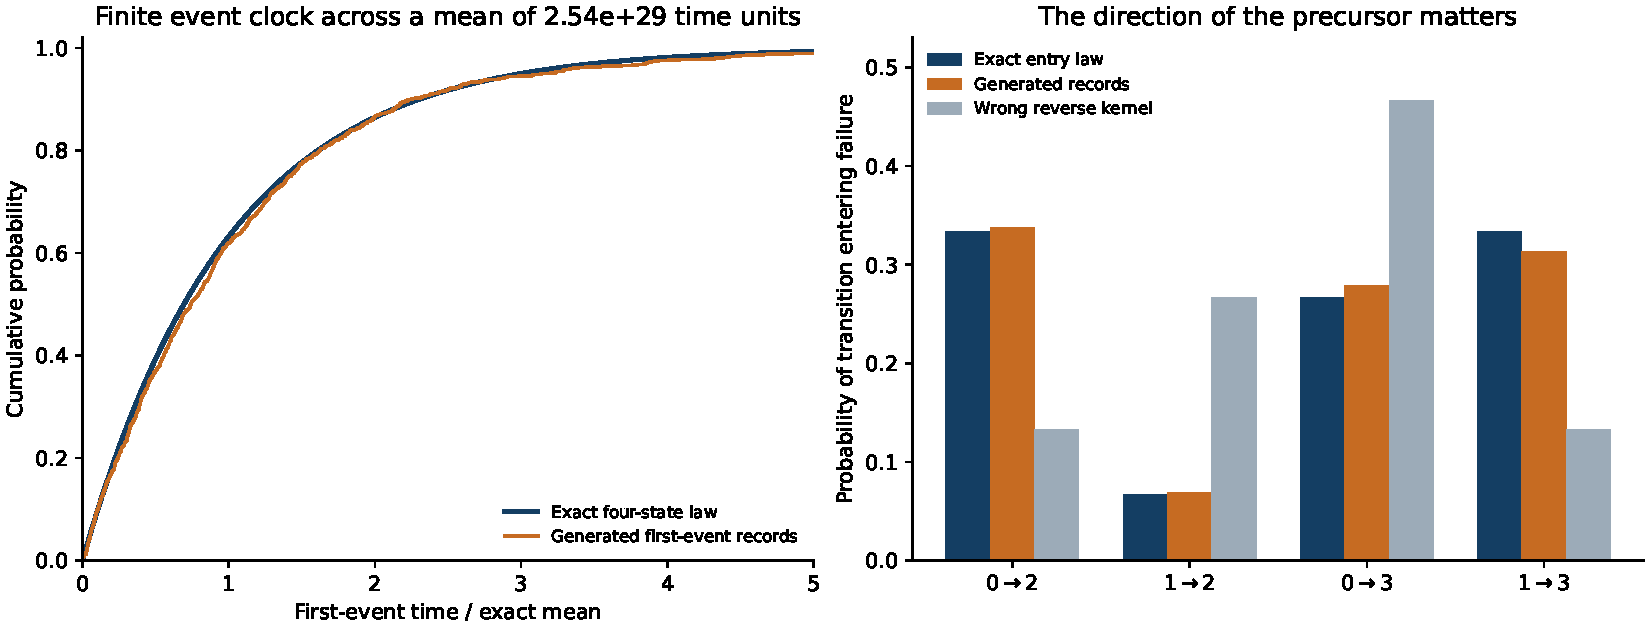
\includegraphics[width=\linewidth]{../next4_execution/event_law_diagnostic.pdf}
\caption{Executed supplied-model diagnostic. Left: generated finite-clock
first-event records against the independent exact law. Right: the entry
transition distribution, including the incorrect boundary reconstruction
that uses the wrong time direction. The small exact solver is a stronger
baseline for this fixture; the plot does not establish practical advantage
for a general exponentially large state space.}
\end{figure}


\section{Preservation and independent destinations}
The preceding 123-file correlated-reliability package is retained byte for byte, including nested passive and deferred calibration packages, all-strength quantum acquisition, the separate global-budget correction, matched parity/GHZ resource law, finite-slew and calibration constructions, thermal effusion with its geometry and exposure bill, reliability curves and their distinct starts, the transport obstruction, passive-memory inequality and useful failed attempts. A before/after hash receipt accompanies the new archive. Originals are unchanged.

Independent constructors owned active model acquisition, exact fixed-law prediction and active thermodynamic identifiability questions before selection. Their full original derivations and source comparisons are retained with their own completion and overlap status. They are not silently made premises of this theorem.

\subsection{Active acquisition and a matching intervention boundary}
The independent active route completes a conditional local-data-to-risk
construction for a known bounded-degree pairwise Gibbs mechanism. Known
neighbor clamps and calibrated compensating fields expose local log odds;
finite holds, readings, field slew and amplitude are priced. The final
construction does not assume that a calibration field preserves an
operating kinetic clock. It prepares a priced focal state and measures the
fast escape separately at every operating context, then uses detailed
balance to reconstruct the slow reverse rate.

An actual finite relaxation-and-safe-rejection preparation yields a
statewise-relative approximation to the equilibrium-safe start. The
earlier changing-law CDF comparison then propagates local factor/rate
confidence and the preparation distortion. The setup requires a repairable
continuing process, all declared variables, faithful clamps/copies,
calibrated fields and positive local relaxation bounds. It does not certify
that a real irreversible catastrophe can be survived during setup.

The matching information bound has exposure proportional to
$e^{(B-H_{\rm field})_+}/(r\eta_{\rm loc}^2)$ when a field cap cannot cancel
a local log-odds barrier $B$, even with adaptive fields and full jump records
under the specified measurement interface. Parameter-independent resets are
granted in that lower bound; field motion is charged in wall time.
The completed source compares active spin-network learning and learning
from Glauber dynamics rather than treating interventions as a new primitive
\cite{jiang,dutt}.

Its four-bit diagnostic used 30,226,360 bit readings and 7,747,360
preparations. The declared single-channel total was
409,497,107.05 model time units. If its rates were per second, this would
be about thirteen years. It is therefore an explicit construction and
resource boundary, not an economical calibration claim. Full proof and
the exact access model are retained in the independent-route source.

\subsection{Exact consistency for a single fixed dynamical law}
The independent mathematical route uses established Lipschitz interpolation
and performance-estimation machinery \cite{ryu}, with exact physical-dimension
qualifications. For one observed transition $f(0)=-e$, $\norm e=1$, a
fixed $L$-Lipschitz map in dimension at least two has the sharp envelope
\[
\sup_f\langle e,f(f(-e))\rangle=
\begin{cases}
-1+L(1+L)/(1+2L),&0\le L\le1/2,\\
L^2-7/8,&L\ge1/2.
\end{cases}
\]
Exact sum-of-squares identities and attaining maps are supplied. At $L=1$,
the value is $1/8$, while the scalar fixed-law value is $-1/3$ and the
specified stepwise outer relaxation gives $1$. The gap comes from retaining
consistency between future transitions of the same map.

For $L<1$, possible equilibria are exactly the intersection of balls
\[
\bigcap_i B\left(
\frac{b_i-L^2a_i}{1-L^2},
\frac{L\norm{b_i-a_i}}{1-L^2}\right)
\quad\text{for data }f(a_i)=b_i.
\]
This gives an actual-dimension second-order-cone formulation for a linear
equilibrium objective and an explicit geometric tail from finite-horizon
to all-time bounds. Low-dimensional rank constraints can remain
nonconvex, and finite observations do not establish the global Lipschitz
prior. General interpolation and Gram methods are established; historical
novelty of the particular sharp envelope is not established.

\subsection{A fixed-mechanics thermodynamic ambiguity}
The independent physical route found substantial prior Astra overlap with
active-port thermodynamic nonidentifiability. Two-temperature Brownian
gyrators are an established physical setting \cite{filliger}. Its retained increment is a
cleaner realization with fixed reciprocal mechanics, unit mobility, bath
directions, port and relaxation rates; only two reservoir temperatures
change. With $A=\operatorname{diag}(1,3)$,
$c=(1,1)^\top/\sqrt2$, $v=(1,-1)^\top/\sqrt2$, set
\[
\Sigma_s=A^{-1}+svv^\top,\qquad
D_s=(A\Sigma_s+\Sigma_sA)/2,\qquad
dX=(-AX+cu)\,dt+\sqrt{2D_s}\,dW.
\]
For $0\le s<4+2\sqrt5$, native stationary starts and output $Y=c^\top X$
give identical complete records under every well-posed causal force
controller. Both state directions are controllable and observable.
At $s=0$ the system is at equilibrium; at $s=4$ it has positive temperatures
$5\pm2\sqrt5$, heat current $4/\sqrt5$, and entropy production $16/5$,
yet the same accessible mechanical transcript.

The unbounded-entropy limit requires a bath temperature tending to zero
and does not imply unbounded heat power. A trusted reset of the full hidden
covariance or an added thermal port breaks the equivalence, but is extra
physical access. Native stationary initialization and ideal white baths
are explicit premises. This is retained as a stricter physical example,
not promoted as a new broad nonidentifiability discovery.

The governing prior publication is pinned at revision
\texttt{fef3640a8b1dc5475674a006de417f652f3baf3c}:
\href{https://github.com/harjassand/astra-research-knowledge/tree/fef3640a8b1dc5475674a006de417f652f3baf3c/research/returns/2026-11-05-p3-correlated-reliability}{Governing correlated-reliability publication}.
Accepted earlier mathematics is used at its stated scope. This work constructs a new operation rather than revalidating those premises.

\begin{thebibliography}{10}
\small
\bibitem{blanchet} J. Blanchet, \emph{Optimal Sampling of Overflow Paths in Jackson Networks}, Mathematics of Operations Research 38 (2013), 698--719. \url{https://doi.org/10.1287/moor.2013.0586}. Author manuscript: \url{https://web.stanford.edu/~jblanche/papers/RareJackson7.pdf}.
\bibitem{koskela} J. Koskela, D. Spano and P. A. Jenkins, \emph{Inference and rare event simulation for stopped Markov processes via reverse-time sequential Monte Carlo}, Statistics and Computing 28 (2018), 131--144. \url{https://doi.org/10.1007/s11222-017-9722-1}.
\bibitem{ops} D. W. H. Swenson et al., \emph{OpenPathSampling: A Python Framework for Path Sampling Simulations. 1. Basics}, J. Chemical Theory and Computation 15 (2019), 813--836. \url{https://doi.org/10.1021/acs.jctc.8b00626}.
\bibitem{we} B. W. Zhang, D. Jasnow and D. M. Zuckerman, \emph{The weighted ensemble path sampling method is statistically exact for a broad class of stochastic processes and binning procedures}, J. Chemical Physics 132 (2010), 054107. \url{https://doi.org/10.1063/1.3306345}.
\bibitem{botev} Z. I. Botev and P. L'Ecuyer, \emph{Sampling Conditionally on a Rare Event via Generalized Splitting}, INFORMS J. Computing 32 (2020), 986--995. \url{https://doi.org/10.1287/ijoc.2019.0936}.
\bibitem{parrep} D. Aristoff, T. Lelievre and G. Simpson, \emph{The Parallel Replica Method for Simulating Long Trajectories of Markov Chains}, Applied Mathematics Research eXpress (2014), 332--352. \url{https://doi.org/10.1093/amrx/abu005}.
\bibitem{aldous} D. Aldous, \emph{Markov chains with almost exponential hitting times}, Stochastic Processes and their Applications 13 (1982), 305--310. \url{https://doi.org/10.1016/0304-4149(82)90016-3}.
\bibitem{zweimuller} R. Zweimuller, \emph{Hitting Times and Positions in Rare Events}, Annales Henri Lebesgue 5 (2022), 1361--1415. \url{https://doi.org/10.5802/ahl.154}.
\bibitem{sharpe} D. J. Sharpe and D. J. Wales, \emph{Numerical analysis of first-passage processes in finite Markov chains exhibiting metastability}, Physical Review E 104 (2021), 015301. \url{https://doi.org/10.1103/PhysRevE.104.015301}.
\bibitem{jiang} J. Jiang, D. A. Sivak and M. Thomson, \emph{Active Learning of Spin Network Models}, arXiv:1903.10474 (2019). \url{https://arxiv.org/abs/1903.10474}.
\bibitem{dutt} A. Dutt, A. Y. Lokhov, M. Vuffray and S. Misra, \emph{Exponential Reduction in Sample Complexity with Learning of Ising Model Dynamics}, Proceedings of Machine Learning Research 139 (2021), 2914--2925. \url{https://proceedings.mlr.press/v139/dutt21a.html}.
\bibitem{ryu} E. K. Ryu, A. B. Taylor, C. Bergeling and P. Giselsson, \emph{Operator Splitting Performance Estimation: Tight Contraction Factors and Optimal Parameter Selection}, arXiv:1812.00146. \url{https://arxiv.org/abs/1812.00146}.
\bibitem{filliger} R. Filliger and P. Reimann, \emph{Brownian Gyrator: A Minimal Heat Engine on the Nanoscale}, Physical Review Letters 99 (2007), 230602. \url{https://doi.org/10.1103/PhysRevLett.99.230602}.
\end{thebibliography}
